% ============================================================================
% CSCE 775: Deep Reinforcement Learning - Homework 1
% ============================================================================

\documentclass[12pt]{article}

% ============================================================================
% PACKAGE IMPORTS
% ============================================================================
\usepackage{amsmath}
\usepackage{graphicx}
\usepackage{amssymb}
\usepackage{tikz}
\usepackage[margin=1in]{geometry}
\usepackage{setspace}
\usepackage{xcolor}
\usepackage{enumitem}
\usepackage{tcolorbox}
\usepackage{fancyhdr}
\usepackage{booktabs}
\usepackage{array}
\usepackage{colortbl}
\usepackage{float}
\usepackage{bm}

% ============================================================================
% HEADER AND FOOTER SETUP
% ============================================================================
\pagestyle{fancy}
\setlength{\headheight}{14.5pt}
\fancyhf{}

\fancyhead[L]{Page \thepage}
\fancyhead[C]{CSCE 775}
\fancyhead[R]{JC Vaught}

\renewcommand{\headrulewidth}{0pt}

% ============================================================================
% TIKZ LIBRARIES
% ============================================================================
\usetikzlibrary{shapes.geometric, arrows.meta, positioning, automata, calc, decorations.markings, patterns}

% --- USC Brand Colors ---
\definecolor{USC_Garnet}{HTML}{73000A}
\definecolor{USC_Sandstorm}{HTML}{FFF2E3}
\definecolor{USC_Black90}{HTML}{363636}
\definecolor{USC_Black70}{HTML}{5C5C5C}
\definecolor{USC_Black50}{HTML}{A2A2A2}
\definecolor{USC_Black10}{HTML}{ECECEC}
\definecolor{USC_Honeycomb}{HTML}{A49137}
\definecolor{USC_Horseshoe}{HTML}{65780B}
\definecolor{USC_Atlantic}{HTML}{466A9F}
\definecolor{USC_Congaree}{HTML}{1F414D}
\definecolor{USC_Rose}{HTML}{CC2E40}

% ============================================================================
% CUSTOM COLORED BOXES
% ============================================================================
\newtcolorbox{stepbox}[1][Step]{
  colback=white,
  colframe=USC_Garnet,
  fonttitle=\bfseries,
  title=#1,
  sharp corners,
  colbacktitle=USC_Garnet,
  coltitle=white,
}

\newtcolorbox{resultsbox}{
  colback=white,
  colframe=USC_Horseshoe,
  fonttitle=\bfseries,
  title=Results,
  sharp corners,
  colbacktitle=USC_Horseshoe,
  coltitle=white,
}

\newtcolorbox{codebox}[1][Code]{
  colback=white,
  colframe=USC_Atlantic,
  fonttitle=\bfseries,
  title=#1,
  sharp corners,
  colbacktitle=USC_Atlantic,
  coltitle=white,
}

% ============================================================================
% CUSTOM QUESTION AND PART COMMANDS
% ============================================================================
\newcommand{\question}[1]{%
  \clearpage
  \vspace{0.5cm}
  {\noindent\normalsize \textbf{#1}}
  \vspace{0.2cm}
  \hrule
  \vspace{0.1cm}
  \hrule
  \vspace{0.3cm}
}

\newcommand{\questionpart}[1]{%
  \clearpage
  \vspace{0.5cm}
  {\noindent\normalsize \textbf{#1}}
  \vspace{0.2cm}
  \hrule
  \vspace{0.1cm}
  \hrule
  \vspace{0.3cm}
}

% ============================================================================
% DOCUMENT INFORMATION
% ============================================================================

\title{CSCE 775: Deep Reinforcement Learning \\ Homework \#1}
\author{Instructor: Dr. Forest Agostinelli \\ University of South Carolina \\ \textit{Solutions by: JC Vaught}}
\date{Spring 2026}

% ============================================================================
% BEGIN DOCUMENT
% ============================================================================

\begin{document}

\maketitle
\setlength{\parindent}{0pt}

\setlist[enumerate,1]{label=\arabic*.}
\setlist[enumerate,2]{label=(\alph*)}

% ============================================================================
% TABLE OF CONTENTS
% ============================================================================

\begin{center}
\begin{tcolorbox}[colback=white, colframe=gray!50!black, colbacktitle=gray!20!white,
                  coltitle=black, sharp corners, boxrule=1pt,
                  title=\Large\bfseries Table of Contents]
\begin{tabular}{p{0.82\textwidth}r}
\textbf{Problem 1: Markov Reward Processes (20 pts)} \dotfill & \textbf{\pageref{quest:mrp}} \\[0.3em]
\textbf{Problem 2: Markov Decision Processes (80 pts)} & \\
\quad 2.1: Dynamic Programming (40 pts) \dotfill & \textbf{\pageref{quest:dp}} \\
\quad 2.2: Model-Free Reinforcement Learning (40 pts) \dotfill & \textbf{\pageref{quest:mf}} \\
\end{tabular}
\vspace{0.2cm}
\end{tcolorbox}
\end{center}

\vspace{0.5cm}

% ============================================================================
% PROBLEM 1: Markov Reward Processes
% ============================================================================

\question{Problem 1: Markov Reward Processes (20 pts)}\label{quest:mrp}

\textbf{Task:} Implement the \texttt{mrp} function. Given the definition of a Markov reward process, compute the state-values (expected future reward) for all states.

\subsection*{MRP Diagram}

\begin{center}
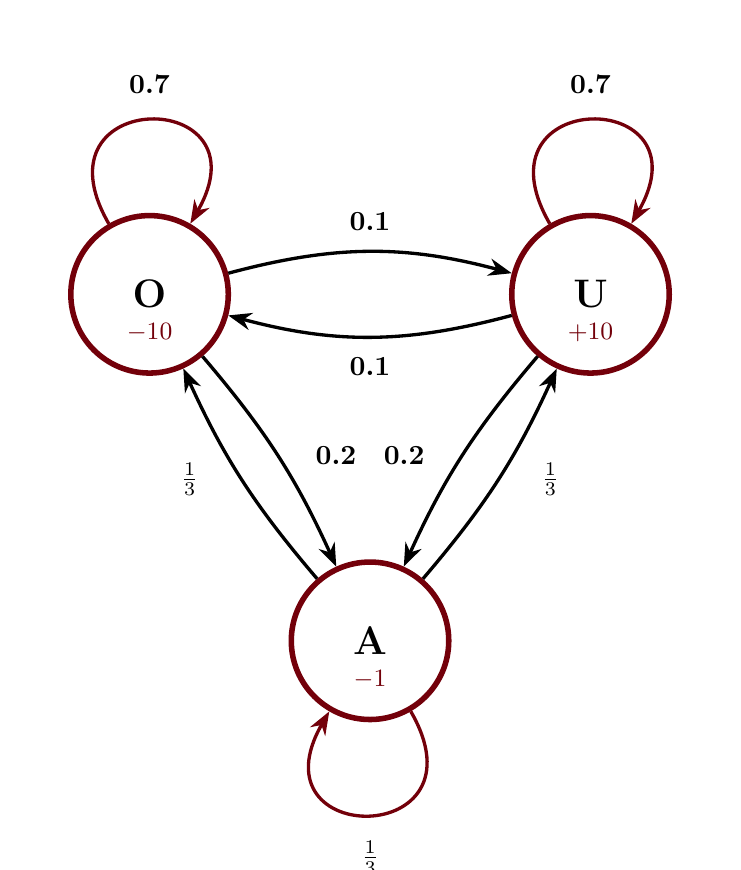
\begin{tikzpicture}[
    >=Stealth,
    scale=0.8,
    every state/.style={
        fill=white,
        draw=USC_Garnet,
        line width=2pt,
        text=black,
        minimum size=2cm,
        font=\bfseries\Large
    },
    every edge/.style={
        draw=black,
        line width=1.2pt,
        ->,
        >=Stealth
    },
    prob/.style={
        font=\bfseries,
        text=black,
        fill=white,
        inner sep=3pt
    },
    statelabel/.style={
        font=\small\bfseries,
        text=USC_Garnet
    }
]

% States
\node[state] (O) at (0, 0) {O};
\node[statelabel, below=1pt of O.center, yshift=-6pt] {$-10$};

\node[state] (U) at (7, 0) {U};
\node[statelabel, below=1pt of U.center, yshift=-6pt] {$+10$};

\node[state] (A) at (3.5, -5.5) {A};
\node[statelabel, below=1pt of A.center, yshift=-6pt] {$-1$};

% Self-loops
\path (O) edge[loop above, looseness=5, out=120, in=60, draw=USC_Garnet] node[prob, above=6pt] {0.7} (O);
\path (U) edge[loop above, looseness=5, out=120, in=60, draw=USC_Garnet] node[prob, above=6pt] {0.7} (U);
\path (A) edge[loop below, looseness=5, out=-60, in=-120, draw=USC_Garnet] node[prob, below=6pt] {$\frac{1}{3}$} (A);

% O <-> U transitions
\path (O) edge[bend left=15] node[prob, above=4pt] {0.1} (U);
\path (U) edge[bend left=15] node[prob, below=4pt] {0.1} (O);

% O <-> A transitions
\path (O) edge[bend left=8] node[prob, right=10pt, pos=0.5] {0.2} (A);
\path (A) edge[bend left=8] node[prob, left=12pt, pos=0.5] {$\frac{1}{3}$} (O);

% U <-> A transitions
\path (U) edge[bend right=8] node[prob, left=10pt, pos=0.5] {0.2} (A);
\path (A) edge[bend right=8] node[prob, right=12pt, pos=0.5] {$\frac{1}{3}$} (U);

\end{tikzpicture}
\end{center}

\subsection*{Problem Formulation}

The state space is $\mathcal{S} = \{O, U, A\}$ with rewards $R(O) = -10$, $R(U) = +10$, $R(A) = -1$.

The transition probability matrix is:
\[
\mathcal{P} = \begin{pmatrix}
0.7 & 0.1 & 0.2 \\
0.1 & 0.7 & 0.2 \\
\frac{1}{3} & \frac{1}{3} & \frac{1}{3}
\end{pmatrix}, \qquad
\mathbf{R} = \begin{pmatrix} -10 \\ +10 \\ -1 \end{pmatrix}
\]

\subsection*{Solution Approach: Matrix Inversion}

\begin{stepbox}[Step 1: Bellman Equation in Matrix Form]
The value function satisfies:
\[
\mathbf{V} = \mathbf{R} + \gamma \mathcal{P} \mathbf{V}
\quad \Longrightarrow \quad
\mathbf{V} = (\mathbf{I} - \gamma \mathcal{P})^{-1} \mathbf{R}
\]
\end{stepbox}

\begin{stepbox}[Step 2: Compute I -- gamma P for gamma = 0.9]
\[
\mathbf{I} - 0.9\mathcal{P} =
\begin{pmatrix} 1 & 0 & 0 \\ 0 & 1 & 0 \\ 0 & 0 & 1 \end{pmatrix}
- 0.9 \begin{pmatrix} 0.7 & 0.1 & 0.2 \\ 0.1 & 0.7 & 0.2 \\ \frac{1}{3} & \frac{1}{3} & \frac{1}{3} \end{pmatrix}
= \begin{pmatrix}
0.37 & -0.09 & -0.18 \\
-0.09 & 0.37 & -0.18 \\
-0.3 & -0.3 & 0.7
\end{pmatrix}
\]
\end{stepbox}

\begin{stepbox}[Step 3: Solve the Linear System]
Computing $\mathbf{V} = (\mathbf{I} - \gamma\mathcal{P})^{-1}\mathbf{R}$ via matrix inversion or a linear solver yields:
\end{stepbox}

\begin{resultsbox}
For $\gamma = 0.9$:
\[
V(O) \approx -23.75, \qquad V(U) \approx +32.01, \qquad V(A) \approx +1.04
\]

\textbf{Interpretation:}
\begin{itemize}[nosep]
    \item $V(O) < 0$: The system tends to stay in $O$ (70\% self-loop), accumulating $-10$ rewards.
    \item $V(U) > 0$: The system tends to stay in $U$ (70\% self-loop), accumulating $+10$ rewards.
    \item $V(A) \approx 0$: Despite the $-1$ reward, there is a $\frac{1}{3}$ chance of reaching the valuable state $U$.
\end{itemize}
\end{resultsbox}

\subsection*{Verification Across Discount Factors}

\begin{center}
\begin{tabular}{cccc}
\toprule
$\bm{\gamma}$ & $\mathbf{V(O)}$ & $\mathbf{V(U)}$ & $\mathbf{V(A)}$ \\
\midrule
0     & $-10.00$ & $+10.00$ & $-1.00$ \\
0.1   & $-10.63$ & $+10.63$ & $-1.00$ \\
0.9   & $-23.75$ & $+32.01$ & $+1.04$ \\
0.999 & $-163.30$ & $+343.37$ & $+88.03$ \\
\bottomrule
\end{tabular}
\end{center}

\begin{codebox}[Implementation]
The \texttt{mrp} function uses NumPy's \texttt{np.linalg.solve} to solve $(\mathbf{I} - \gamma\mathcal{P})\mathbf{V} = \mathbf{R}$:
\begin{verbatim}
import numpy as np

def mrp(P, R, gamma):
    I = np.eye(P.shape[0])
    return np.linalg.solve(I - gamma * P, R)
\end{verbatim}
\end{codebox}

% ============================================================================
% PROBLEM 2.1: Dynamic Programming
% ============================================================================

\question{Problem 2.1: Dynamic Programming (40 pts)}\label{quest:dp}

\textbf{Task:} Implement the \texttt{dynamic\_programming} function. Use any tabular dynamic programming algorithm to exactly compute the optimal state-value function and an optimal policy for the AI Farm environment.

\subsection*{Algorithm: Value Iteration}

Value iteration repeatedly applies the Bellman optimality update until convergence:
\[
V_{k+1}(s) = \max_{a \in \mathcal{A}(s)} \left[ r(s,a) + \gamma \sum_{s'} P(s'|s,a) \cdot V_k(s') \right]
\]

The optimal policy is then:
\[
\pi^*(s) = \arg\max_{a \in \mathcal{A}(s)} \left[ r(s,a) + \gamma \sum_{s'} P(s'|s,a) \cdot V(s') \right]
\]

\begin{stepbox}[Step 1: Initialize]
Set $V(s) = 0$ for all states $s$. Choose convergence threshold $\theta = 10^{-8}$.
\end{stepbox}

\begin{stepbox}[Step 2: Value Iteration Loop]
For each state $s$ and each action $a$:
\begin{enumerate}[nosep]
    \item Call \texttt{env.state\_action\_dynamics(s, a)} to get $r(s,a)$, next states $\{s'\}$, and probabilities $\{P(s'|s,a)\}$.
    \item Compute $Q(s,a) = r(s,a) + \gamma \sum_{s'} P(s'|s,a) \cdot V(s')$.
    \item Update $V(s) = \max_a Q(s,a)$.
\end{enumerate}
Repeat until $\max_s |V_{\text{new}}(s) - V_{\text{old}}(s)| < \theta$.
\end{stepbox}

\begin{stepbox}[Step 3: Extract Policy]
For each state $s$, compute the action probabilities. For the greedy deterministic policy, assign probability 1 to $\arg\max_a Q(s,a)$ and 0 to all other actions.
\end{stepbox}

\subsection*{Worked Example: 2-State MDP}

Consider a simple MDP with states $S_0, S_1$ and terminal state $S_T$, $\gamma = 1$:

\begin{center}
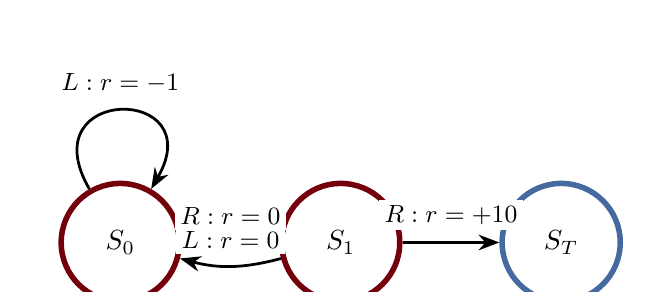
\begin{tikzpicture}[
    >=Stealth,
    scale=0.7,
    every state/.style={
        fill=white,
        draw=USC_Garnet,
        line width=2pt,
        text=black,
        minimum size=1.5cm,
        font=\bfseries
    },
    every edge/.style={draw=black, line width=1pt, ->, >=Stealth},
    prob/.style={font=\small\bfseries, fill=white, inner sep=2pt}
]
\node[state] (S0) at (0, 0) {$S_0$};
\node[state] (S1) at (4, 0) {$S_1$};
\node[state, draw=USC_Atlantic] (ST) at (8, 0) {$S_T$};

\path (S0) edge[loop above, looseness=5, out=120, in=60] node[prob, above=4pt] {$L: r=-1$} (S0);
\path (S0) edge node[prob, above=4pt] {$R: r=0$} (S1);
\path (S1) edge[bend left=15] node[prob, above=4pt] {$L: r=0$} (S0);
\path (S1) edge node[prob, above=4pt] {$R: r=+10$} (ST);
\end{tikzpicture}
\end{center}

\textbf{Value Iteration:}

\begin{center}
\begin{tabular}{ccccl}
\toprule
\textbf{Iter} & $\mathbf{V(S_0)}$ & $\mathbf{V(S_1)}$ & $\bm{\pi(S_0)}$ & $\bm{\pi(S_1)}$ \\
\midrule
0 & 0 & 0 & --- & --- \\
1 & 0 & 10 & R & R \\
2 & 10 & 10 & R & R \\
3 & 10 & 10 & R & R \\
\bottomrule
\end{tabular}
\end{center}

\begin{resultsbox}
Converged: $V^*(S_0) = 10$, $V^*(S_1) = 10$. Optimal policy: $S_0 \to \text{right} \to S_1 \to \text{right} \to S_T$ collecting $+10$ reward.
\end{resultsbox}

\begin{codebox}[Implementation Sketch]
\begin{verbatim}
def dynamic_programming(env, states, state_values, gamma):
    theta = 1e-8
    while True:
        delta = 0
        for s in states:
            actions = env.get_actions(s)
            if not actions:
                continue
            v_old = state_values[s]
            q_values = []
            for a in actions:
                r, next_states, probs = env.state_action_dynamics(s, a)
                q = r + gamma * sum(p * state_values[ns]
                                    for ns, p in zip(next_states, probs))
                q_values.append(q)
            state_values[s] = max(q_values)
            delta = max(delta, abs(v_old - state_values[s]))
        if delta < theta:
            break

    # Extract policy
    policy = {}
    for s in states:
        actions = env.get_actions(s)
        action_probs = [0.0] * len(actions)
        if actions:
            best_q = float('-inf')
            best_idx = 0
            for i, a in enumerate(actions):
                r, next_states, probs = env.state_action_dynamics(s, a)
                q = r + gamma * sum(p * state_values[ns]
                                    for ns, p in zip(next_states, probs))
                if q > best_q:
                    best_q = q
                    best_idx = i
            action_probs[best_idx] = 1.0
        policy[s] = action_probs

    return state_values, policy
\end{verbatim}
\end{codebox}

% ============================================================================
% PROBLEM 2.2: Model-Free RL
% ============================================================================

\question{Problem 2.2: Model-Free Reinforcement Learning (40 pts)}\label{quest:mf}

\textbf{Task:} Implement the \texttt{model\_free} function. Use a tabular model-free RL algorithm to approximate the optimal action-value function. \textbf{Cannot} use \texttt{env.state\_action\_dynamics}.

\subsection*{Algorithm: Q-Learning}

Q-learning is an off-policy TD control algorithm. The update rule is:
\[
Q(s,a) \leftarrow Q(s,a) + \alpha \Big[ r + \gamma \max_{a'} Q(s', a') - Q(s,a) \Big]
\]

with $\varepsilon$-greedy exploration:
\[
a = \begin{cases}
\arg\max_a Q(s,a) & \text{with probability } 1 - \varepsilon \\
\text{random action} & \text{with probability } \varepsilon
\end{cases}
\]

\begin{stepbox}[Step 1: Initialize]
Set $Q(s,a) = 0$ for all state-action pairs. Choose hyperparameters:
\begin{itemize}[nosep]
    \item Learning rate $\alpha \in (0, 1]$ (e.g., $\alpha = 0.1$)
    \item Exploration rate $\varepsilon \in (0, 1]$ (e.g., $\varepsilon = 0.3$, decaying)
    \item Number of episodes (e.g., $N = 10000$)
\end{itemize}
\end{stepbox}

\begin{stepbox}[Step 2: Episode Loop]
For each episode:
\begin{enumerate}[nosep]
    \item Sample start state $s \leftarrow$ \texttt{env.sample\_start\_state()}.
    \item While $s$ is not terminal:
    \begin{enumerate}[nosep]
        \item Select action $a$ via $\varepsilon$-greedy w.r.t. $Q(s, \cdot)$.
        \item Take action: $(s', r) \leftarrow$ \texttt{env.sample\_transition(s, a)}.
        \item Update: $Q(s,a) \leftarrow Q(s,a) + \alpha [r + \gamma \max_{a'} Q(s',a') - Q(s,a)]$.
        \item $s \leftarrow s'$.
    \end{enumerate}
\end{enumerate}
\end{stepbox}

\subsection*{Worked Example: 2-State MDP with Q-Learning}

Same 2-state MDP as before. $\alpha = 0.1$, $\gamma = 1.0$, $\varepsilon = 0.3$.

Initialize: $Q(S_0, L) = Q(S_0, R) = Q(S_1, L) = Q(S_1, R) = 0$.

\begin{stepbox}[Episode 1]
\begin{tabular}{cccccl}
\toprule
\textbf{Step} & $\mathbf{s}$ & $\mathbf{a}$ & $\mathbf{s'}$ & $\mathbf{r}$ & \textbf{Q-update} \\
\midrule
1 & $S_0$ & $R$ & $S_1$ & 0 & $Q(S_0,R) = 0 + 0.1[0 + 0 - 0] = 0$ \\
2 & $S_1$ & $R$ & $S_T$ & 10 & $Q(S_1,R) = 0 + 0.1[10 + 0 - 0] = 1.0$ \\
\bottomrule
\end{tabular}
\end{stepbox}

\begin{stepbox}[Episode 2]
\begin{tabular}{cccccl}
\toprule
\textbf{Step} & $\mathbf{s}$ & $\mathbf{a}$ & $\mathbf{s'}$ & $\mathbf{r}$ & \textbf{Q-update} \\
\midrule
1 & $S_0$ & $R$ & $S_1$ & 0 & $Q(S_0,R) = 0 + 0.1[0 + 1.0 - 0] = 0.1$ \\
2 & $S_1$ & $R$ & $S_T$ & 10 & $Q(S_1,R) = 1.0 + 0.1[10 + 0 - 1.0] = 1.9$ \\
\bottomrule
\end{tabular}
\end{stepbox}

\begin{stepbox}[Episode 3]
\begin{tabular}{cccccl}
\toprule
\textbf{Step} & $\mathbf{s}$ & $\mathbf{a}$ & $\mathbf{s'}$ & $\mathbf{r}$ & \textbf{Q-update} \\
\midrule
1 & $S_0$ & $R$ & $S_1$ & 0 & $Q(S_0,R) = 0.1 + 0.1[0 + 1.9 - 0.1] = 0.28$ \\
2 & $S_1$ & $R$ & $S_T$ & 10 & $Q(S_1,R) = 1.9 + 0.1[10 + 0 - 1.9] = 2.71$ \\
\bottomrule
\end{tabular}
\end{stepbox}

\begin{resultsbox}
After many episodes: $Q(S_0, R) \to 10$, $Q(S_1, R) \to 10$, matching the DP solution.

The greedy policy $\pi(s) = \arg\max_a Q(s,a)$ yields $S_0 \to R$, $S_1 \to R$.
\end{resultsbox}

\begin{codebox}[Implementation Sketch]
\begin{verbatim}
import random

def model_free(env, action_values, gamma):
    alpha = 0.1
    epsilon = 1.0
    epsilon_decay = 0.9995
    epsilon_min = 0.01
    num_episodes = 50000

    for ep in range(num_episodes):
        state = env.sample_start_state()
        while True:
            actions = env.get_actions(state)
            if not actions:
                break
            # Epsilon-greedy
            if random.random() < epsilon:
                idx = random.randrange(len(actions))
            else:
                idx = max(range(len(actions)),
                         key=lambda i: action_values[state][i])
            action = actions[idx]
            next_state, reward = env.sample_transition(state, action)

            # Q-learning update
            next_actions = env.get_actions(next_state)
            max_q_next = max(action_values[next_state]) if next_actions else 0.0
            td_target = reward + gamma * max_q_next
            td_error = td_target - action_values[state][idx]
            action_values[state][idx] += alpha * td_error

            state = next_state

        epsilon = max(epsilon_min, epsilon * epsilon_decay)

    return action_values
\end{verbatim}
\end{codebox}

% ============================================================================
% END OF DOCUMENT
% ============================================================================

\end{document}
